\chapter{Conclusion}
\minitoc
\section{Recap}
The goal of this thesis was to investigate how well the GIRG model can match real graphs with some suspected inherent geometry and power law degree distribution.

Our first attempt was to follow the framework of \cite{blasius2018towards}, to compare a range of generative graph models, including many GIRG subtypes, in their ability to replicate global statistics of a set of ~100 social network graphs.
In this arena we did find GIRGs able to outperform on a few statistics: closeness centrality, Katz centrality, effective diameter, and average local clustering coefficient. 

We then explored fitting GIRG location parameters to these real graphs to see if they're capable of replicating the real graphs on an edge level. This found a decent amount of success.

We tried to use graph kernels in a bayesian framework for assessing evidence of GIRG models against Chung-Lu as generative models of the real graphs. However graph kernels proved incapable of correctly identifying the generative model even when the assessed graph was generated by the same model. Hence we abandoned this avenue.





% \begin{figure}
%   \centering
% 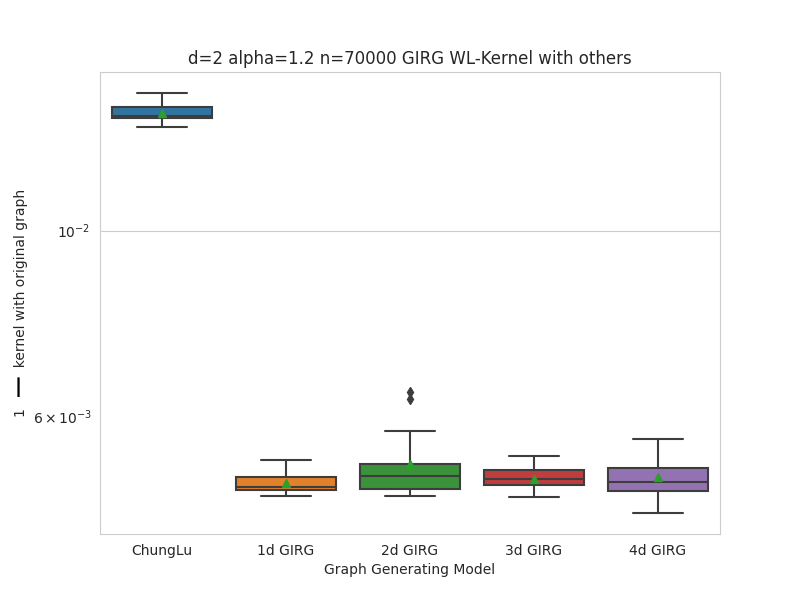
\includegraphics[width=0.8\linewidth]{figures/d=2 alpha=1.2 n=70000 GIRG WL-Kernel with others.png}
% \caption{WL-Kernel of a d=2, alpha=1.2, n=70000 Torus GIRG with other generated graphs (13 per model). All the GIRGs are more similar to the original than Chung-Lu, but we cannot differentiate between different GIRGs.}
% \label{fig:wl_kernel_gentorus}
% \end{figure}

% socfb-Brandeis99 d=3.png


% \begin{figure}
%   \centering
% 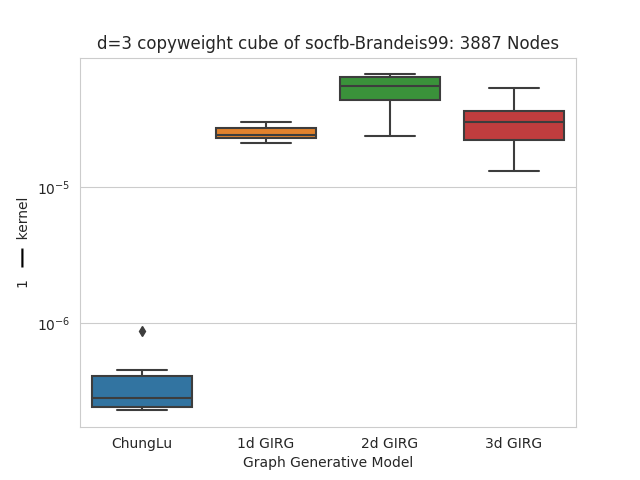
\includegraphics[width=0.8\linewidth]{figures/socfb-Brandeis99 d=3.png}
% \caption{RW-Kernel of a d=3 copy weight cube GIRG fit to socfb-Brandeis99 (matching number of edges and local clustering coefficient), with other generated graphs (6 per model type). Chung-Lu graphs have highest similarity to the original, despite it being a 3D GIRG}
% \label{fig:rw_kernel_fitcopycube}
% \end{figure}


